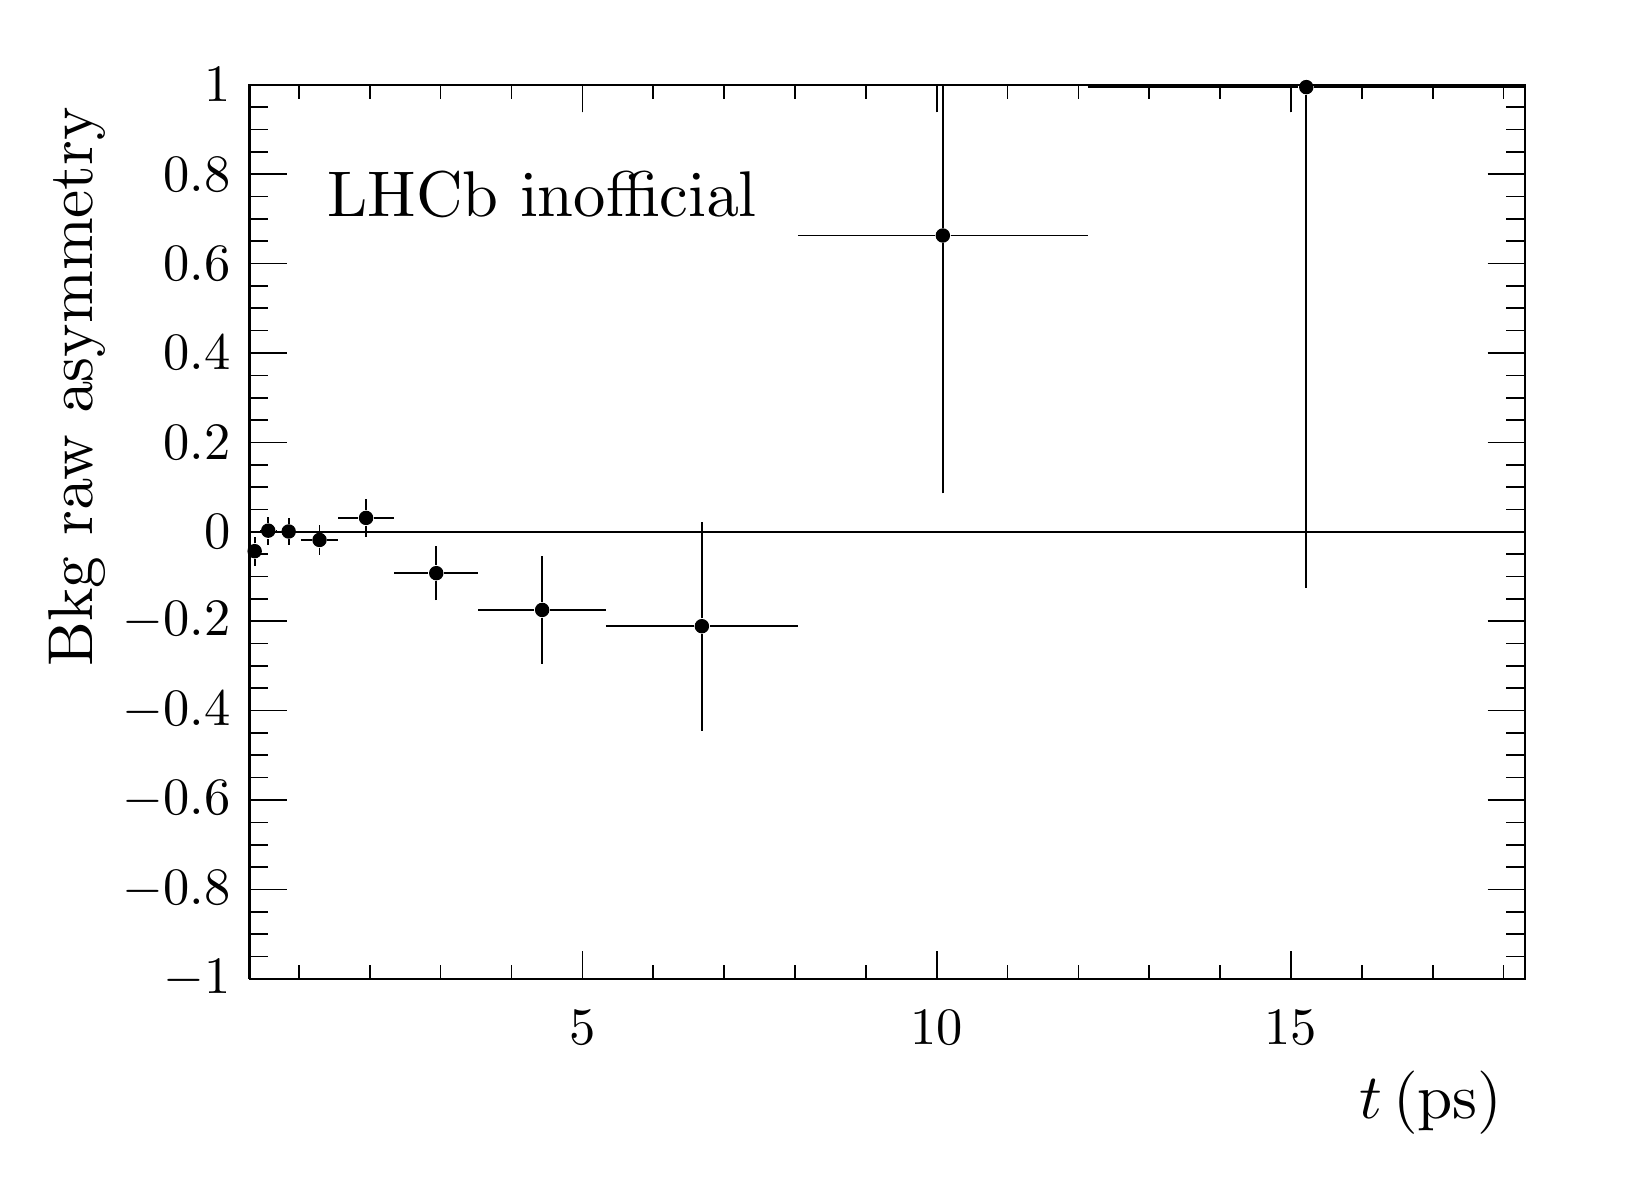
\begin{tikzpicture}
\pgfdeclareplotmark{cross} {
\pgfpathmoveto{\pgfpoint{-0.3\pgfplotmarksize}{\pgfplotmarksize}}
\pgfpathlineto{\pgfpoint{+0.3\pgfplotmarksize}{\pgfplotmarksize}}
\pgfpathlineto{\pgfpoint{+0.3\pgfplotmarksize}{0.3\pgfplotmarksize}}
\pgfpathlineto{\pgfpoint{+1\pgfplotmarksize}{0.3\pgfplotmarksize}}
\pgfpathlineto{\pgfpoint{+1\pgfplotmarksize}{-0.3\pgfplotmarksize}}
\pgfpathlineto{\pgfpoint{+0.3\pgfplotmarksize}{-0.3\pgfplotmarksize}}
\pgfpathlineto{\pgfpoint{+0.3\pgfplotmarksize}{-1.\pgfplotmarksize}}
\pgfpathlineto{\pgfpoint{-0.3\pgfplotmarksize}{-1.\pgfplotmarksize}}
\pgfpathlineto{\pgfpoint{-0.3\pgfplotmarksize}{-0.3\pgfplotmarksize}}
\pgfpathlineto{\pgfpoint{-1.\pgfplotmarksize}{-0.3\pgfplotmarksize}}
\pgfpathlineto{\pgfpoint{-1.\pgfplotmarksize}{0.3\pgfplotmarksize}}
\pgfpathlineto{\pgfpoint{-0.3\pgfplotmarksize}{0.3\pgfplotmarksize}}
\pgfpathclose
\pgfusepathqstroke
}
\pgfdeclareplotmark{cross*} {
\pgfpathmoveto{\pgfpoint{-0.3\pgfplotmarksize}{\pgfplotmarksize}}
\pgfpathlineto{\pgfpoint{+0.3\pgfplotmarksize}{\pgfplotmarksize}}
\pgfpathlineto{\pgfpoint{+0.3\pgfplotmarksize}{0.3\pgfplotmarksize}}
\pgfpathlineto{\pgfpoint{+1\pgfplotmarksize}{0.3\pgfplotmarksize}}
\pgfpathlineto{\pgfpoint{+1\pgfplotmarksize}{-0.3\pgfplotmarksize}}
\pgfpathlineto{\pgfpoint{+0.3\pgfplotmarksize}{-0.3\pgfplotmarksize}}
\pgfpathlineto{\pgfpoint{+0.3\pgfplotmarksize}{-1.\pgfplotmarksize}}
\pgfpathlineto{\pgfpoint{-0.3\pgfplotmarksize}{-1.\pgfplotmarksize}}
\pgfpathlineto{\pgfpoint{-0.3\pgfplotmarksize}{-0.3\pgfplotmarksize}}
\pgfpathlineto{\pgfpoint{-1.\pgfplotmarksize}{-0.3\pgfplotmarksize}}
\pgfpathlineto{\pgfpoint{-1.\pgfplotmarksize}{0.3\pgfplotmarksize}}
\pgfpathlineto{\pgfpoint{-0.3\pgfplotmarksize}{0.3\pgfplotmarksize}}
\pgfpathclose
\pgfusepathqfillstroke
}
\pgfdeclareplotmark{newstar} {
\pgfpathmoveto{\pgfqpoint{0pt}{\pgfplotmarksize}}
\pgfpathlineto{\pgfqpointpolar{44}{0.5\pgfplotmarksize}}
\pgfpathlineto{\pgfqpointpolar{18}{\pgfplotmarksize}}
\pgfpathlineto{\pgfqpointpolar{-20}{0.5\pgfplotmarksize}}
\pgfpathlineto{\pgfqpointpolar{-54}{\pgfplotmarksize}}
\pgfpathlineto{\pgfqpointpolar{-90}{0.5\pgfplotmarksize}}
\pgfpathlineto{\pgfqpointpolar{234}{\pgfplotmarksize}}
\pgfpathlineto{\pgfqpointpolar{198}{0.5\pgfplotmarksize}}
\pgfpathlineto{\pgfqpointpolar{162}{\pgfplotmarksize}}
\pgfpathlineto{\pgfqpointpolar{134}{0.5\pgfplotmarksize}}
\pgfpathclose
\pgfusepathqstroke
}
\pgfdeclareplotmark{newstar*} {
\pgfpathmoveto{\pgfqpoint{0pt}{\pgfplotmarksize}}
\pgfpathlineto{\pgfqpointpolar{44}{0.5\pgfplotmarksize}}
\pgfpathlineto{\pgfqpointpolar{18}{\pgfplotmarksize}}
\pgfpathlineto{\pgfqpointpolar{-20}{0.5\pgfplotmarksize}}
\pgfpathlineto{\pgfqpointpolar{-54}{\pgfplotmarksize}}
\pgfpathlineto{\pgfqpointpolar{-90}{0.5\pgfplotmarksize}}
\pgfpathlineto{\pgfqpointpolar{234}{\pgfplotmarksize}}
\pgfpathlineto{\pgfqpointpolar{198}{0.5\pgfplotmarksize}}
\pgfpathlineto{\pgfqpointpolar{162}{\pgfplotmarksize}}
\pgfpathlineto{\pgfqpointpolar{134}{0.5\pgfplotmarksize}}
\pgfpathclose
\pgfusepathqfillstroke
}
\definecolor{c}{rgb}{1,1,1};
\draw [color=c, fill=c] (0,0) rectangle (20,14.3719);
\draw [color=c, fill=c] (2.8,2.2995) rectangle (19,13.6533);
\definecolor{c}{rgb}{0,0,0};
\draw [c,line width=0.9] (2.8,2.2995) -- (2.8,13.6533) -- (19,13.6533) -- (19,2.2995) -- (2.8,2.2995);
\definecolor{c}{rgb}{1,1,1};
\draw [color=c, fill=c] (2.8,2.2995) rectangle (19,13.6533);
\definecolor{c}{rgb}{0,0,0};
\draw [c,line width=0.9] (2.8,2.2995) -- (2.8,13.6533) -- (19,13.6533) -- (19,2.2995) -- (2.8,2.2995);
\draw [c,line width=0.6] (2.86864,7.54798) -- (2.86864,7.62992);
\draw [c,line width=0.6] (2.86864,7.83093) -- (2.86864,7.91287);
\foreach \P in {(2.86864,7.73042)}{\draw[mark options={color=c,fill=c},mark size=2.402402pt,mark=*] plot coordinates {\P};}
\draw [c,line width=0.6] (3.04083,7.81287) -- (3.04083,7.89046);
\draw [c,line width=0.6] (3.04083,8.09147) -- (3.04083,8.16906);
\draw [c,line width=0.6] (2.93728,7.99096) -- (2.94032,7.99096);
\draw [c,line width=0.6] (3.14133,7.99096) -- (3.14437,7.99096);
\foreach \P in {(3.04083,7.99096)}{\draw[mark options={color=c,fill=c},mark size=2.402402pt,mark=*] plot coordinates {\P};}
\draw [c,line width=0.6] (3.30056,7.81197) -- (3.30056,7.87991);
\draw [c,line width=0.6] (3.30056,8.08091) -- (3.30056,8.14885);
\draw [c,line width=0.6] (3.14437,7.98041) -- (3.20006,7.98041);
\draw [c,line width=0.6] (3.40106,7.98041) -- (3.45675,7.98041);
\foreach \P in {(3.30056,7.98041)}{\draw[mark options={color=c,fill=c},mark size=2.402402pt,mark=*] plot coordinates {\P};}
\draw [c,line width=0.6] (3.69236,7.68555) -- (3.69236,7.77251);
\draw [c,line width=0.6] (3.69236,7.97351) -- (3.69236,8.06047);
\draw [c,line width=0.6] (3.45675,7.87301) -- (3.59185,7.87301);
\draw [c,line width=0.6] (3.79286,7.87301) -- (3.92796,7.87301);
\foreach \P in {(3.69236,7.87301)}{\draw[mark options={color=c,fill=c},mark size=2.402402pt,mark=*] plot coordinates {\P};}
\draw [c,line width=0.6] (4.28337,7.9092) -- (4.28337,8.05244);
\draw [c,line width=0.6] (4.28337,8.25344) -- (4.28337,8.39668);
\draw [c,line width=0.6] (3.92796,8.15294) -- (4.18286,8.15294);
\draw [c,line width=0.6] (4.38387,8.15294) -- (4.63877,8.15294);
\foreach \P in {(4.28337,8.15294)}{\draw[mark options={color=c,fill=c},mark size=2.402402pt,mark=*] plot coordinates {\P};}
\draw [c,line width=0.6] (5.17488,7.10946) -- (5.17488,7.35065);
\draw [c,line width=0.6] (5.17488,7.55166) -- (5.17488,7.79285);
\draw [c,line width=0.6] (4.63877,7.45116) -- (5.07437,7.45116);
\draw [c,line width=0.6] (5.27538,7.45116) -- (5.71099,7.45116);
\foreach \P in {(5.17488,7.45116)}{\draw[mark options={color=c,fill=c},mark size=2.402402pt,mark=*] plot coordinates {\P};}
\draw [c,line width=0.6] (6.51968,6.29917) -- (6.51968,6.88363);
\draw [c,line width=0.6] (6.51968,7.08464) -- (6.51968,7.6691);
\draw [c,line width=0.6] (5.71099,6.98414) -- (6.41918,6.98414);
\draw [c,line width=0.6] (6.62019,6.98414) -- (7.32838,6.98414);
\foreach \P in {(6.51968,6.98414)}{\draw[mark options={color=c,fill=c},mark size=2.402402pt,mark=*] plot coordinates {\P};}
\draw [c,line width=0.6] (8.54827,5.44929) -- (8.54827,6.67702);
\draw [c,line width=0.6] (8.54827,6.87803) -- (8.54827,8.10576);
\draw [c,line width=0.6] (7.32838,6.77753) -- (8.44776,6.77753);
\draw [c,line width=0.6] (8.64877,6.77753) -- (9.76815,6.77753);
\foreach \P in {(8.54827,6.77753)}{\draw[mark options={color=c,fill=c},mark size=2.402402pt,mark=*] plot coordinates {\P};}
\draw [c,line width=0.6] (11.6083,8.46425) -- (11.6083,11.6388);
\draw [c,line width=0.6] (11.6083,11.8398) -- (11.6083,13.6533);
\draw [c,line width=0.6] (9.76815,11.7393) -- (11.5078,11.7393);
\draw [c,line width=0.6] (11.7088,11.7393) -- (13.4484,11.7393);
\foreach \P in {(11.6083,11.7393)}{\draw[mark options={color=c,fill=c},mark size=2.402402pt,mark=*] plot coordinates {\P};}
\draw [c,line width=0.6] (16.2242,7.2632) -- (16.2242,13.5234);
\draw [c,line width=0.6] (13.4484,13.6239) -- (16.1237,13.6239);
\draw [c,line width=0.6] (16.3247,13.6239) -- (19,13.6239);
\foreach \P in {(16.2242,13.6239)}{\draw[mark options={color=c,fill=c},mark size=2.402402pt,mark=*] plot coordinates {\P};}
\draw [c,line width=0.6] (2.8,2.2995) -- (19,2.2995);
\draw [anchor= east] (19,0.726641) node[scale=2.28793, color=c, rotate=0]{$t\,\mathrm{(ps)}$};
\draw [c,line width=0.6] (7.03,2.64873) -- (7.03,2.2995);
\draw [c,line width=0.6] (7.93,2.47412) -- (7.93,2.2995);
\draw [c,line width=0.6] (8.83,2.47412) -- (8.83,2.2995);
\draw [c,line width=0.6] (9.73,2.47412) -- (9.73,2.2995);
\draw [c,line width=0.6] (10.63,2.47412) -- (10.63,2.2995);
\draw [c,line width=0.6] (11.53,2.64873) -- (11.53,2.2995);
\draw [c,line width=0.6] (12.43,2.47412) -- (12.43,2.2995);
\draw [c,line width=0.6] (13.33,2.47412) -- (13.33,2.2995);
\draw [c,line width=0.6] (14.23,2.47412) -- (14.23,2.2995);
\draw [c,line width=0.6] (15.13,2.47412) -- (15.13,2.2995);
\draw [c,line width=0.6] (16.03,2.64873) -- (16.03,2.2995);
\draw [c,line width=0.6] (7.03,2.64873) -- (7.03,2.2995);
\draw [c,line width=0.6] (6.13,2.47412) -- (6.13,2.2995);
\draw [c,line width=0.6] (5.23,2.47412) -- (5.23,2.2995);
\draw [c,line width=0.6] (4.33,2.47412) -- (4.33,2.2995);
\draw [c,line width=0.6] (3.43,2.47412) -- (3.43,2.2995);
\draw [c,line width=0.6] (16.03,2.64873) -- (16.03,2.2995);
\draw [c,line width=0.6] (16.93,2.47412) -- (16.93,2.2995);
\draw [c,line width=0.6] (17.83,2.47412) -- (17.83,2.2995);
\draw [c,line width=0.6] (18.73,2.47412) -- (18.73,2.2995);
\draw [anchor=base] (7.03,1.46593) node[scale=1.89731, color=c, rotate=0]{5};
\draw [anchor=base] (11.53,1.46593) node[scale=1.89731, color=c, rotate=0]{10};
\draw [anchor=base] (16.03,1.46593) node[scale=1.89731, color=c, rotate=0]{15};
\draw [c,line width=0.6] (2.8,13.6533) -- (19,13.6533);
\draw [c,line width=0.6] (7.03,13.304) -- (7.03,13.6533);
\draw [c,line width=0.6] (7.93,13.4786) -- (7.93,13.6533);
\draw [c,line width=0.6] (8.83,13.4786) -- (8.83,13.6533);
\draw [c,line width=0.6] (9.73,13.4786) -- (9.73,13.6533);
\draw [c,line width=0.6] (10.63,13.4786) -- (10.63,13.6533);
\draw [c,line width=0.6] (11.53,13.304) -- (11.53,13.6533);
\draw [c,line width=0.6] (12.43,13.4786) -- (12.43,13.6533);
\draw [c,line width=0.6] (13.33,13.4786) -- (13.33,13.6533);
\draw [c,line width=0.6] (14.23,13.4786) -- (14.23,13.6533);
\draw [c,line width=0.6] (15.13,13.4786) -- (15.13,13.6533);
\draw [c,line width=0.6] (16.03,13.304) -- (16.03,13.6533);
\draw [c,line width=0.6] (7.03,13.304) -- (7.03,13.6533);
\draw [c,line width=0.6] (6.13,13.4786) -- (6.13,13.6533);
\draw [c,line width=0.6] (5.23,13.4786) -- (5.23,13.6533);
\draw [c,line width=0.6] (4.33,13.4786) -- (4.33,13.6533);
\draw [c,line width=0.6] (3.43,13.4786) -- (3.43,13.6533);
\draw [c,line width=0.6] (16.03,13.304) -- (16.03,13.6533);
\draw [c,line width=0.6] (16.93,13.4786) -- (16.93,13.6533);
\draw [c,line width=0.6] (17.83,13.4786) -- (17.83,13.6533);
\draw [c,line width=0.6] (18.73,13.4786) -- (18.73,13.6533);
\draw [c,line width=0.6] (2.8,2.2995) -- (2.8,13.6533);
\draw [anchor= east] (0.6112,13.6533) node[scale=2.28793, color=c, rotate=90]{Bkg raw asymmetry};
\draw [c,line width=0.6] (3.274,2.2995) -- (2.8,2.2995);
\draw [c,line width=0.6] (3.037,2.58334) -- (2.8,2.58334);
\draw [c,line width=0.6] (3.037,2.86719) -- (2.8,2.86719);
\draw [c,line width=0.6] (3.037,3.15103) -- (2.8,3.15103);
\draw [c,line width=0.6] (3.274,3.43487) -- (2.8,3.43487);
\draw [c,line width=0.6] (3.037,3.71872) -- (2.8,3.71872);
\draw [c,line width=0.6] (3.037,4.00256) -- (2.8,4.00256);
\draw [c,line width=0.6] (3.037,4.28641) -- (2.8,4.28641);
\draw [c,line width=0.6] (3.274,4.57025) -- (2.8,4.57025);
\draw [c,line width=0.6] (3.037,4.8541) -- (2.8,4.8541);
\draw [c,line width=0.6] (3.037,5.13794) -- (2.8,5.13794);
\draw [c,line width=0.6] (3.037,5.42178) -- (2.8,5.42178);
\draw [c,line width=0.6] (3.274,5.70563) -- (2.8,5.70563);
\draw [c,line width=0.6] (3.037,5.98947) -- (2.8,5.98947);
\draw [c,line width=0.6] (3.037,6.27332) -- (2.8,6.27332);
\draw [c,line width=0.6] (3.037,6.55716) -- (2.8,6.55716);
\draw [c,line width=0.6] (3.274,6.84101) -- (2.8,6.84101);
\draw [c,line width=0.6] (3.037,7.12485) -- (2.8,7.12485);
\draw [c,line width=0.6] (3.037,7.40869) -- (2.8,7.40869);
\draw [c,line width=0.6] (3.037,7.69254) -- (2.8,7.69254);
\draw [c,line width=0.6] (3.274,7.97638) -- (2.8,7.97638);
\draw [c,line width=0.6] (3.037,8.26023) -- (2.8,8.26023);
\draw [c,line width=0.6] (3.037,8.54407) -- (2.8,8.54407);
\draw [c,line width=0.6] (3.037,8.82791) -- (2.8,8.82791);
\draw [c,line width=0.6] (3.274,9.11176) -- (2.8,9.11176);
\draw [c,line width=0.6] (3.037,9.3956) -- (2.8,9.3956);
\draw [c,line width=0.6] (3.037,9.67945) -- (2.8,9.67945);
\draw [c,line width=0.6] (3.037,9.96329) -- (2.8,9.96329);
\draw [c,line width=0.6] (3.274,10.2471) -- (2.8,10.2471);
\draw [c,line width=0.6] (3.037,10.531) -- (2.8,10.531);
\draw [c,line width=0.6] (3.037,10.8148) -- (2.8,10.8148);
\draw [c,line width=0.6] (3.037,11.0987) -- (2.8,11.0987);
\draw [c,line width=0.6] (3.274,11.3825) -- (2.8,11.3825);
\draw [c,line width=0.6] (3.037,11.6664) -- (2.8,11.6664);
\draw [c,line width=0.6] (3.037,11.9502) -- (2.8,11.9502);
\draw [c,line width=0.6] (3.037,12.234) -- (2.8,12.234);
\draw [c,line width=0.6] (3.274,12.5179) -- (2.8,12.5179);
\draw [c,line width=0.6] (3.037,12.8017) -- (2.8,12.8017);
\draw [c,line width=0.6] (3.037,13.0856) -- (2.8,13.0856);
\draw [c,line width=0.6] (3.037,13.3694) -- (2.8,13.3694);
\draw [c,line width=0.6] (3.274,13.6533) -- (2.8,13.6533);
\draw [c,line width=0.6] (3.274,2.2995) -- (2.8,2.2995);
\draw [anchor= east] (2.8,2.2995) node[scale=1.89731, color=c, rotate=0]{$-1$};
\draw [anchor= east] (2.8,3.43487) node[scale=1.89731, color=c, rotate=0]{$-0.8$};
\draw [anchor= east] (2.8,4.57025) node[scale=1.89731, color=c, rotate=0]{$-0.6$};
\draw [anchor= east] (2.8,5.70563) node[scale=1.89731, color=c, rotate=0]{$-0.4$};
\draw [anchor= east] (2.8,6.84101) node[scale=1.89731, color=c, rotate=0]{$-0.2$};
\draw [anchor= east] (2.8,7.97638) node[scale=1.89731, color=c, rotate=0]{$0$};
\draw [anchor= east] (2.8,9.11176) node[scale=1.89731, color=c, rotate=0]{$0.2$};
\draw [anchor= east] (2.8,10.2471) node[scale=1.89731, color=c, rotate=0]{$0.4$};
\draw [anchor= east] (2.8,11.3825) node[scale=1.89731, color=c, rotate=0]{$0.6$};
\draw [anchor= east] (2.8,12.5179) node[scale=1.89731, color=c, rotate=0]{$0.8$};
\draw [anchor= east] (2.8,13.6533) node[scale=1.89731, color=c, rotate=0]{$1$};
\draw [c,line width=0.6] (19,2.2995) -- (19,13.6533);
\draw [c,line width=0.6] (18.526,2.2995) -- (19,2.2995);
\draw [c,line width=0.6] (18.763,2.58334) -- (19,2.58334);
\draw [c,line width=0.6] (18.763,2.86719) -- (19,2.86719);
\draw [c,line width=0.6] (18.763,3.15103) -- (19,3.15103);
\draw [c,line width=0.6] (18.526,3.43487) -- (19,3.43487);
\draw [c,line width=0.6] (18.763,3.71872) -- (19,3.71872);
\draw [c,line width=0.6] (18.763,4.00256) -- (19,4.00256);
\draw [c,line width=0.6] (18.763,4.28641) -- (19,4.28641);
\draw [c,line width=0.6] (18.526,4.57025) -- (19,4.57025);
\draw [c,line width=0.6] (18.763,4.8541) -- (19,4.8541);
\draw [c,line width=0.6] (18.763,5.13794) -- (19,5.13794);
\draw [c,line width=0.6] (18.763,5.42178) -- (19,5.42178);
\draw [c,line width=0.6] (18.526,5.70563) -- (19,5.70563);
\draw [c,line width=0.6] (18.763,5.98947) -- (19,5.98947);
\draw [c,line width=0.6] (18.763,6.27332) -- (19,6.27332);
\draw [c,line width=0.6] (18.763,6.55716) -- (19,6.55716);
\draw [c,line width=0.6] (18.526,6.84101) -- (19,6.84101);
\draw [c,line width=0.6] (18.763,7.12485) -- (19,7.12485);
\draw [c,line width=0.6] (18.763,7.40869) -- (19,7.40869);
\draw [c,line width=0.6] (18.763,7.69254) -- (19,7.69254);
\draw [c,line width=0.6] (18.526,7.97638) -- (19,7.97638);
\draw [c,line width=0.6] (18.763,8.26023) -- (19,8.26023);
\draw [c,line width=0.6] (18.763,8.54407) -- (19,8.54407);
\draw [c,line width=0.6] (18.763,8.82791) -- (19,8.82791);
\draw [c,line width=0.6] (18.526,9.11176) -- (19,9.11176);
\draw [c,line width=0.6] (18.763,9.3956) -- (19,9.3956);
\draw [c,line width=0.6] (18.763,9.67945) -- (19,9.67945);
\draw [c,line width=0.6] (18.763,9.96329) -- (19,9.96329);
\draw [c,line width=0.6] (18.526,10.2471) -- (19,10.2471);
\draw [c,line width=0.6] (18.763,10.531) -- (19,10.531);
\draw [c,line width=0.6] (18.763,10.8148) -- (19,10.8148);
\draw [c,line width=0.6] (18.763,11.0987) -- (19,11.0987);
\draw [c,line width=0.6] (18.526,11.3825) -- (19,11.3825);
\draw [c,line width=0.6] (18.763,11.6664) -- (19,11.6664);
\draw [c,line width=0.6] (18.763,11.9502) -- (19,11.9502);
\draw [c,line width=0.6] (18.763,12.234) -- (19,12.234);
\draw [c,line width=0.6] (18.526,12.5179) -- (19,12.5179);
\draw [c,line width=0.6] (18.763,12.8017) -- (19,12.8017);
\draw [c,line width=0.6] (18.763,13.0856) -- (19,13.0856);
\draw [c,line width=0.6] (18.763,13.3694) -- (19,13.3694);
\draw [c,line width=0.6] (18.526,13.6533) -- (19,13.6533);
\draw [c,line width=0.6] (18.526,2.2995) -- (19,2.2995);
\draw [c,line width=0.6] (2.881,7.97638) -- (3.043,7.97638) -- (3.205,7.97638) -- (3.367,7.97638) -- (3.529,7.97638) -- (3.691,7.97638) -- (3.853,7.97638) -- (4.015,7.97638) -- (4.177,7.97638) -- (4.339,7.97638) -- (4.501,7.97638) -- (4.663,7.97638)
 -- (4.825,7.97638) -- (4.987,7.97638) -- (5.149,7.97638) -- (5.311,7.97638) -- (5.473,7.97638) -- (5.635,7.97638) -- (5.797,7.97638) -- (5.959,7.97638) -- (6.121,7.97638) -- (6.283,7.97638) -- (6.445,7.97638) -- (6.607,7.97638) -- (6.769,7.97638) --
 (6.931,7.97638) -- (7.093,7.97638) -- (7.255,7.97638) -- (7.417,7.97638) -- (7.579,7.97638) -- (7.741,7.97638) -- (7.903,7.97638) -- (8.065,7.97638) -- (8.227,7.97638) -- (8.389,7.97638) -- (8.551,7.97638) -- (8.713,7.97638) -- (8.875,7.97638) --
 (9.037,7.97638) -- (9.199,7.97638) -- (9.361,7.97638) -- (9.523,7.97638) -- (9.685,7.97638) -- (9.847,7.97638) -- (10.009,7.97638) -- (10.171,7.97638) -- (10.333,7.97638) -- (10.495,7.97638) -- (10.657,7.97638) -- (10.819,7.97638);
\draw [c,line width=0.6] (10.819,7.97638) -- (10.981,7.97638) -- (11.143,7.97638) -- (11.305,7.97638) -- (11.467,7.97638) -- (11.629,7.97638) -- (11.791,7.97638) -- (11.953,7.97638) -- (12.115,7.97638) -- (12.277,7.97638) -- (12.439,7.97638) --
 (12.601,7.97638) -- (12.763,7.97638) -- (12.925,7.97638) -- (13.087,7.97638) -- (13.249,7.97638) -- (13.411,7.97638) -- (13.573,7.97638) -- (13.735,7.97638) -- (13.897,7.97638) -- (14.059,7.97638) -- (14.221,7.97638) -- (14.383,7.97638) --
 (14.545,7.97638) -- (14.707,7.97638) -- (14.869,7.97638) -- (15.031,7.97638) -- (15.193,7.97638) -- (15.355,7.97638) -- (15.517,7.97638) -- (15.679,7.97638) -- (15.841,7.97638) -- (16.003,7.97638) -- (16.165,7.97638) -- (16.327,7.97638) --
 (16.489,7.97638) -- (16.651,7.97638) -- (16.813,7.97638) -- (16.975,7.97638) -- (17.137,7.97638) -- (17.299,7.97638) -- (17.461,7.97638) -- (17.623,7.97638) -- (17.785,7.97638) -- (17.947,7.97638) -- (18.109,7.97638) -- (18.271,7.97638) --
 (18.433,7.97638) -- (18.595,7.97638) -- (18.757,7.97638);
\draw [c,line width=0.6] (18.757,7.97638) -- (18.919,7.97638);
\definecolor{c}{rgb}{0,0,0};
\draw [c, anchor=base west, align=left] (3.5,11) node[scale=2.33383, color=c, rotate=0]{LHCb inofficial\\\BdToJPsiKS};
\end{tikzpicture}
